
\subsection{SLA Model}

An rSLA document describes how metrics are to be obtained from instrumentation and how they are to be aggregated. Based on those metrics Service Level Objectives (SLOs) can be defined and it can be specified how to proceed if those SLOs are met or violated. 
The following figure \ref{fig:concepts} illustrates the main concepts of the proposed approach using a simple example.

\begin{figure}[H]
\centering
 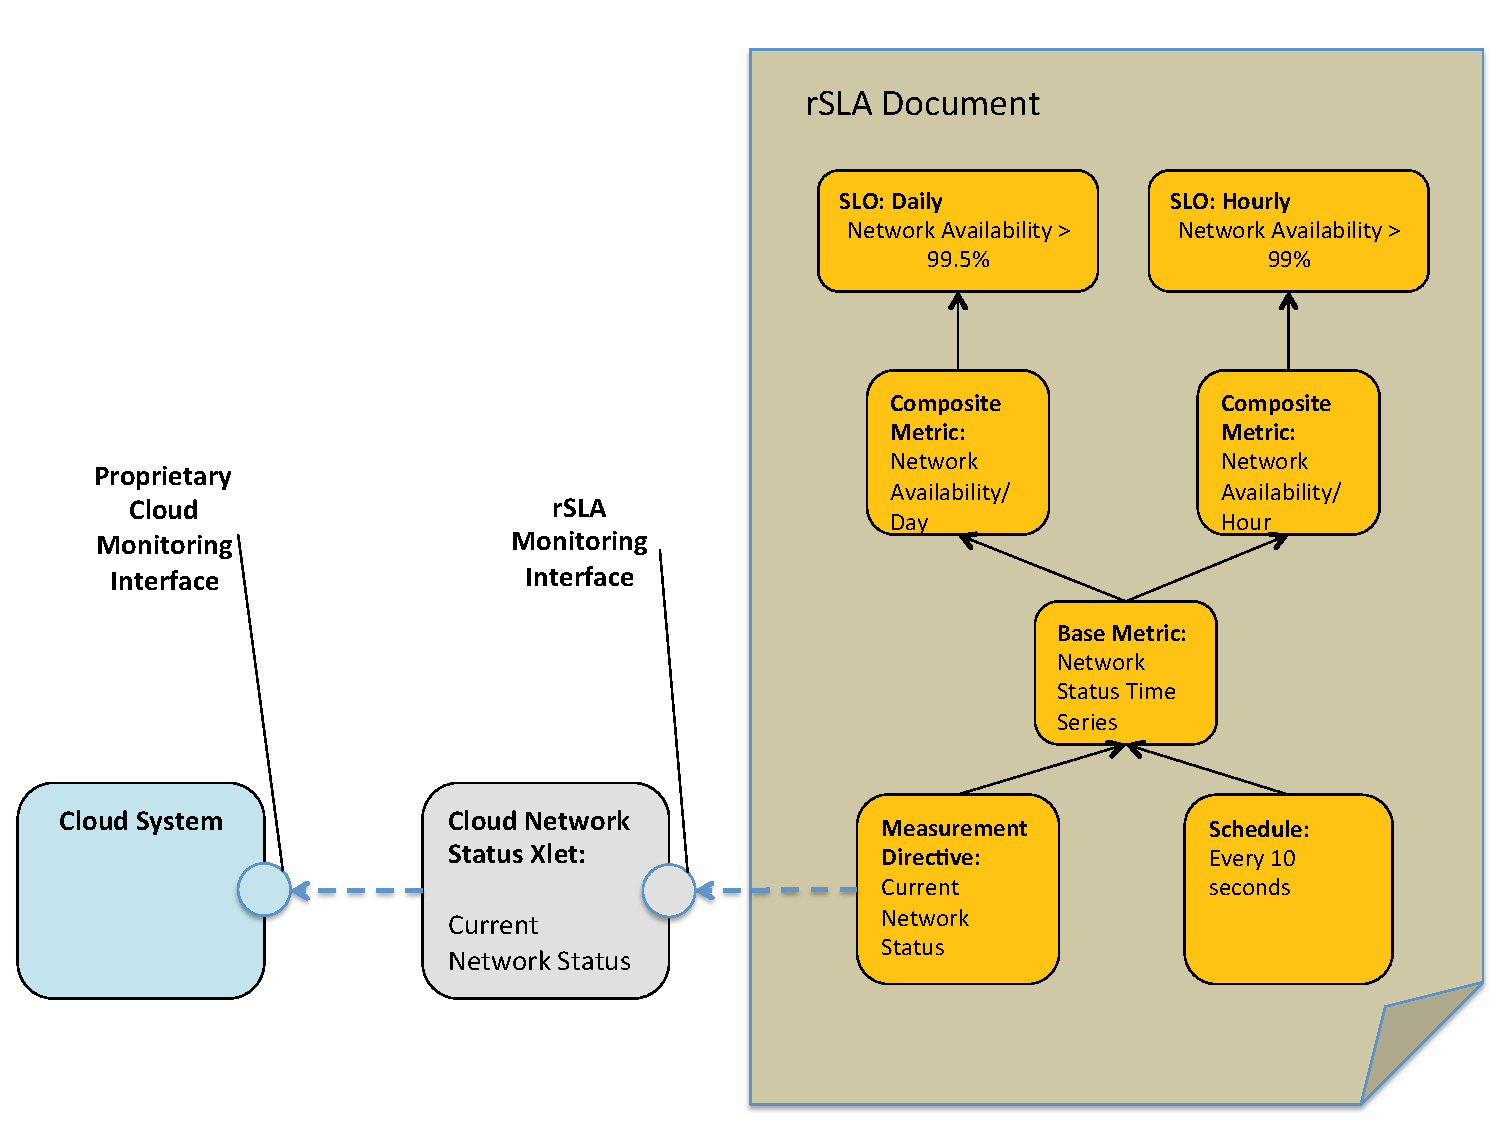
\includegraphics[width=\textwidth]{pics/concepts.pdf} 
 \caption{rSLA Concepts Overview}
 \label{fig:concepts}
\end{figure}

This example describes an SLA defining networking guarantees. The customer is interested in a daily guarantee, which needs to exceed 99.5\% availability, and an hourly, which needs to be only 99\%. The current status of the network at any given point in time can be obtained at the proprietary interface of the Cloud provider with whom the customer enters the SLA. There is an xlet exposing an rSLA monitoring interface that can be requested to provide network status in an rSLA standard way and which in turns requests this status from the proprietary Cloud management interface. 

When expressing the rSLA document the author of this document has to describe how what can be read by instrumentation can be translated into a high-level metric on which the customer wants to have a commitment. In addition, the actual SLO must be articulated. This gives us our main set of concepts for rSLA:

The foundation of measurement are {\em base metrics}. Base metrics describe how metrics are to be obtained from instrumentation and how frequently. For this purpose a base metric has a measurement directive and a schedule.

The {\em measurement directive} describes how a specific metric can be obtained through an xlet. It points to an xlet and the specific system element and metric that needs to be obtained. For example, our networking xlet for this Cloud provider may provider status for an extenal access network as well as an internal network, between the different virtual machines of this customer. Multiple metrics may be available such as availability, latency and jitter. The measurement directive will point to the specific metric of a specific entity.

The {\em schedule} describes the frequency at which measurements are taken. The periodicity can reflect the customer's needs. For our networking example this time frame will typically be a sampling interval in a range of seconds to a minute or two.

{\em Composite metrics} aggregate values of base metrics and other composite metrics. The aggregations are described using expressions over values from those metrics it depends on. The phrasing of the expression must be type-compatible with the types of the input metrics. Oftentimes, expressions involve aggregations of time series, e.g. to averages over a time period, or aggegregate different metrics such as the network availability of the network of one sebment and the availability of another. In our example, two composite metrics depend on the same base metric, one aggregating network state in the window of the last hour, one in the window of a day. While the basic approach to metric aggregation is simple, we often find quite complex functions excluding some values and performing complex stochastic operations. This puts significant requirements on the richness of the expression language that the language provides.

{\em Service Level Objectives} define the commitment of a service provider to its customer. This is defined in a Boolean expression over metric values. Oftentimes, commitments are bounded by a precondition. For example, a response time guarantee for a ReST call is only given if the request rate to the service is less than a certain number of calls per minute. This is commonly used to scope the applicability of the SLO. Service level objectives can also be associated with a schedule that defines when to evaluate the precondition and objective expressions. Alternatively, it can be evaluated each time input metrics have new values. This might lead to significant computation when large numbers of metrics are sampled at high frequency.

Finally, though not shown in the figure, {\em notifications} define how external services are to be informed about the state of SLOs and metrics. The rSLA language provides notifications as event-condition-action rules that describe when notifications should take place, according to a schedule or when a new evaluation is available; the specific condition, e.g., upon violation; and how to notify. For this how part, the action, we fall back to our xlet concept. Notification xlets provide a homogenous interface abstracting from various possible recepient interfaces. Notification directives describe how to connect to those xlets. Notification statements also include a description which information is to be passed on.

Based on this small set of concepts SLA authors can express a large variety of SLAs. Measurement directives connect the rSLA language to the systems model; composite metrics can express custom metrics aggregation to the level needed by the client; SLOs express the commitment; Notifications define how to actively communicate the SLO status and other information to recepient services.



\section{rSLA Language}\label{language}

The rSLA language allows an SLA author to express the concepts outlined in the previous section. The specific language design is key to the consumability of the language and the usability of the approach as a whole. Prior to diving into the specifics of our language elements we want to briefly discuss some issues and guiding principles.

\subsection{Design considerations}

Many of past and current approaches to representing SLAs such as WSLA, WS-Agreement, WSOL and CSLA choose XML as a substrate. While some of those languages have enjoyed success in systems deployment or as basis for further research work none has seen wide-spread adoption in industry at this point. While not having systematically studied adoption, the authors of this paper have been involved in some of those efforts and received feedback as to why or why not to use one language or another. A key item of feedback from practitioners was that XML is hard to read. While there is always the opportunity to provide advanced editors to not expose authors to the actual representation many professionals actually prefer writing system-level scripts in their intended representation.

When considering who would actually writes rSLA documents it turns out that this would often be admistrators with significant experience in scripting. The rSLA syntax is designed to resemble other languages that administrators use on a daily basis. Many domain specific languages have seen acceptance lately, e.g., Chef. rSLA aims at providing a similar experience to its authors.

Another issue with early efforts such as WSLA is the limitation of its expression language, or its complete absence, in case of WS-Agreement. While WSLA has an extensible set of functions a practitioner would have to change its evaluation engine to extend it. This is not practical. WS-Agreement suggests to use the expression language of your choice, again requiring an addition to a runtime system. From a practioner's perspective they are incomplete. The rSLA langauge is meant to encompass a wide set of functions that can be used in expressions. In addition, the language design enables to define extension to the standard language expression scope as part of the SLA document itself.

To achieve those objectives the rSLA language is designed as a Domain Specific Language (DSL) on the basis of Ruby. Ruby, as a substrate language, has some characteristics that makes it suitable as a basis of a DSL, in particular its scripting approach and its easy access to meta-interpretation. Many DSLs such as Chef are also based on Ruby and many administrators have encountered them before. Other languages and their interpreters might be equally suitable from a technical requirements perspective. 


\subsection{rSLA language elements}\label{editing}

This section discusses the rSLA language elements in an overiew and example manner. We provide a small  rSLA document that specifies three rSLA objects: an rSLA, a base metric and a service level objective. The SLA can be read by an rSLA engine in a cloud runtime environment. A full description of the language is beyond the scope of an individual paper. The rSLA language documentation describes in detail the language structure, the use of rSLA statements and production rules \cite{rSLAspec}.
Listings \ref{basescript} and \ref{sloscript} illustrate example statements for the creation of an SLA and a base metric and respectively of an SLO object. A deployed rSLA service can read and process these statements in a runtime environment. 

An rSLA document must have exactly one $sla$ statement. The $sla$ statement defines the parties to the SLA. 



\begin{minipage}{1.0\textwidth}
\begin{lstlisting}[language=Ruby, basicstyle=\small\normalfont\sffamily, breaklines=true,  captionpos=b, mathescape=true, caption=rSLA SLA (lines 1-4) and basemetric (lines 6-19)  statements, label=basescript, numbers=left, numbersep=5pt, numberstyle=\tiny] 
sla do
  tenant "ExampleClient"
  provider "ExampleProvider"
end  

basemetric do
    name "bareMetalProvisioning"
    unit "seconds"
    type "event_set integer"

    measurementdirective do
    	entity "/process/baremetal_provisioning"
    	type "event_set integer"
    	source "http://provisioningxlet.stage1.mybluemix.net/process/baremetal_provisioning/time" 
    end

    schedule do
    	frequency "1"
   	unit "m"
   	method "every"
    end
end
\end{lstlisting}
\end{minipage} 

The base metric definition includes its $measurementdirective$ and may include a $schedule$ if values are received according to a schedule. Its attributes are $name$,  $unit$ and $type$. 

The type of this particular example is an $event\_set$ of $integer$. Types of metrics can be either simple types or one of two complex types: $time_series$ and $event\_set$. An event set is a set of values collected over time. Typical examples are provisioning events. In a given time interval any number of provisioning processes may have occurred. If a provider wants to give a guarantee over the time it takes to provision, say for 90 \% of the processes, we need a complex type able to accommodate this set of values representing the time it took. Time series, on the other hand, are aequidistant readings of values. 

The measurement directive describes where to read the base metric's values. It describes the entity in question, its type, and the source. In this specific case the source is a fully articulated URL. Based on detailed metric name and entity specification a reference to an xlet name could have sufficed as well.

The schedule follows the syntax of the Rufus scheduler, which is sufficient for our purposes (Citation).

Another required element of an SLA is the SLO. An example of such an SLO statement is illustrated by Listing \ref{sloscript}.

\begin{minipage}{1.0\textwidth}
\begin{lstlisting}[language=Ruby, basicstyle=\small\normalfont\sffamily, breaklines=true,  captionpos=b, mathescape=true, caption=rSLA SLO creation script, label=sloscript, numbers=left, numbersep=5pt, numberstyle=\tiny] 
slo do
    name "bareMetalProvisioning"
    precondition "bmtotalProvisionsNumber.value <= 100"
    objective "bmGoodProvisionsNumber.value) / bmtotalProvisionsNumber.value >= 0.9"

    schedule do
       frequency "60"
       unit "m"
       method "every"
    end
end 
\end{lstlisting}
\end{minipage}

The SLO definition in Listing \ref{sloscript} provides an example of an SLO statement in the rSLA language. The $slo$ has a name to refer to, a schedule according to which it is evaluated and two expressions: the $precondition$ defines the bounding condition of the SLO while the $objective$ defines what must bee achieved.

On SLO evaluation, the rSLA engine will first evaluate the precondition block. If the logical outcome from the execution of the precondition block is false, the SLO is met. In our case, if the total number of mare metal servers provisioned in the past hour is less or equal than hundred, the SLO applies. If it is larger, it doesn't - and no violation occurs. In case the precondition is true or if there is no precondition block, the rSLA runtime will proceed with the evaluation of the objective block. If the logical outcome from processing the statements in the objective block is true, then the SLO is healthy. Otherwise the SLO evaluation indicates not-healthy. A non-healthy SLO may result into a violation. 

Both BaseMetric and SLO programming blocks enable a  user to define schedules for the measurement and respectively the evaluation of such rSLA instances. Schedule details are passed to a backend scheduler service that instantiates such schedule objects and coordinates their processing. We will discuss further details on schduling later in the paper.

Both precondition and objective are expressions following Ruby syntax. Values of metrics, both base metrics and composite metrics, are referred to by their name "." value. This can refer to a complex type or a simple type. Ruby expressions resolving to a Boolean type are valid. This enables authors to use any available Ruby function, providing the full expressiveness of the substrate scripting language.  

Not illustrated for space reasons is the $composite\_metric$ statement. It has name, unit and type like the $base\_metric$ but rather than a measurement directive it has an expression as well, which has to yield a result according to its type. Equally, all type-compatible Ruby expressions are valid.

This syntax allows administrators and others of similar skill to define SLAs in a scripting-like DSL. Using an existing scripting language as substrate, in our case Ruby, enables us to use a full scope of expressions.


%\subsection{Conceptual model}
%In an rSLA runtime environment a service is described by its provisioning compliance levels, which in turn are decomposed into multifarious service level management elements. The rSLA language follows the semantic decomposition of the WSLA specification \cite{wsla}, where an SLA takes the form of a directed graph that has a single root vertex. The root node is connected to three vertices that denote primary branches of the hierarchical tree. 
%
%In an rSLA tree, the root vertex represents a single SLA object. An SLA can be defined by sets of base, composite metrics and SLO objects. Figure \ref{rslaobject} illustrates programming objects of the rSLA language. Connections between such objects compose an rSLA tree. Figure \ref{rslagraph} formalizes an rSLA tree as a directed graph and highlights immediate attributes of rSLA objects.
%
%As illustrated in Figure \ref{rslagraph} an rSLA tree can be defined by a set of vertices $V$ and a set of edges $E$, where vertices represent rSLA tree branches and edges connections between such branches. The set of SLA vertices in an rSLA tree contains exactly one SLA object and one or more base metrics and service level objectives. The SLA object represents the root of the directed graph. 
%
%There is no overlapping between rSLA language objects. Conceptually every object is related to other rSLA objects for the processing of SLA management operations. 
% 
%%\begin{figure}[!ht]
%%    \subfloat[rSLA vocabulary formalization\label{rslagraph}]{%
%%      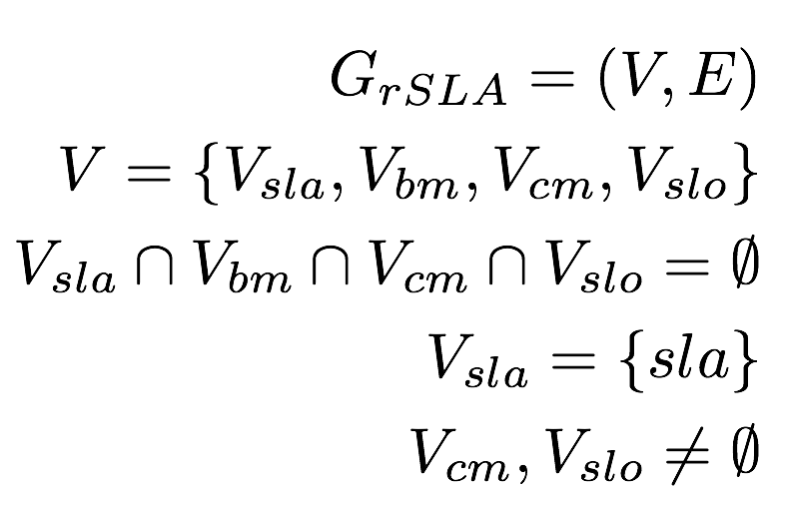
\includegraphics[width=0.45\textwidth]{pics/rslagraph.png}
%%    }
%%    \hfill
%%    \subfloat[rSLA object tree\label{rslaobject}]{%
%%      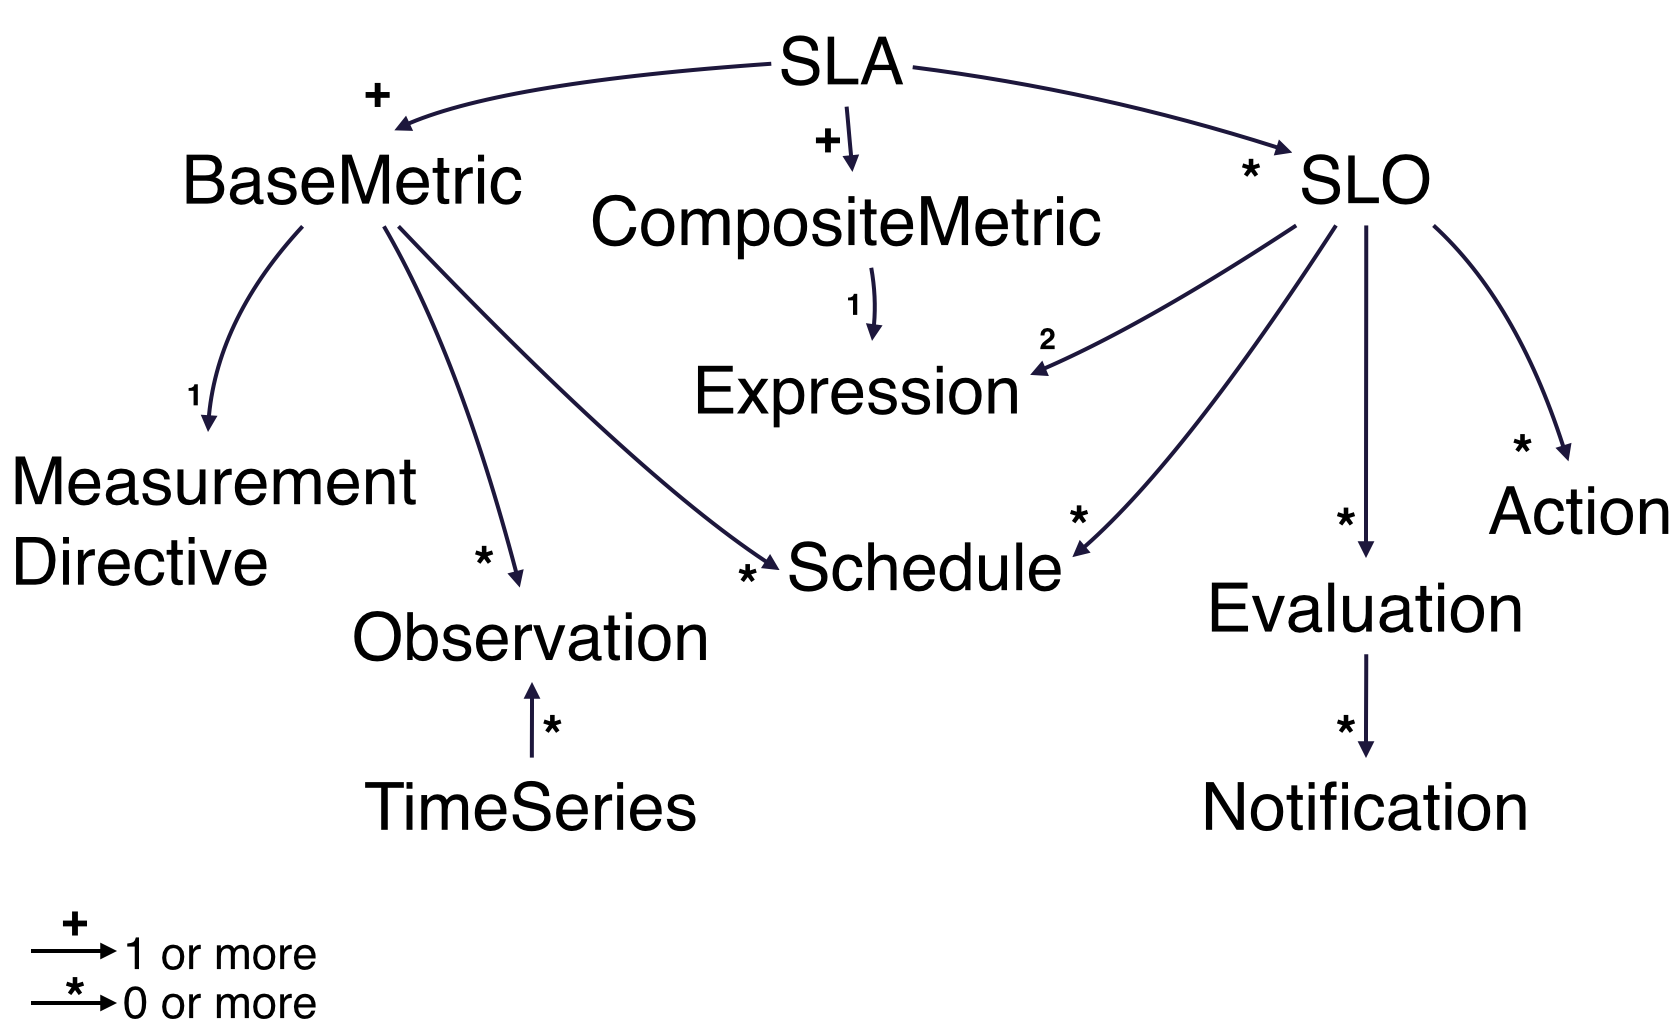
\includegraphics[width=0.45\textwidth]{pics/rslaobject.png}
%%    }
%%    \caption{rSLA vocabulary}\label{treegraph}
%%  \end{figure} 
%
%Nodes that are close to the tree root in Figure \ref{rslaobject}, designate SLA branches like base, composite metrics and service level objectives. Edges between nodes are uni-directed to illustrate the rSLA tree hierarchy. The edge direction points to the nested element in the hierarchical relationship. 
%Edges are labeled with +, * or number symbols to indicate the multiplicity of nested objects. 
%
%In an rSLA runtime environment, a base metric is represented by a restful endpoint that designates a URI source for reading metric data values. A base metric is also described by sets of time-series data-values that are derived during metric measurement. On the other hand, a composite metric represents the computation result from combining either a single pair of data values or multiple data value sets. 
%
%In the rSLA alphabet nested relationships denote inclusive associations between objects. For example, an SLA includes base, composite metrics as well as SLOs. As shown in Figure \ref{rslaobject}, edges between  rSLA objects do not share the same multiplicity rules. 
%
%rSLA notification and timeSeries objects are not initially required to create and activate SLA instances in an rSLA aware environment, but they may be required while one or more SLA management tasks are processed. Such objects are created by service level management operations like monitoring data analysis or automated notification reports on scheduled events of service level evaluation. 
%
%The rSLA DSL exposes such objects as structured programming blocks that a user can edit and customize according to specific needs. A user can introduce new elements in the rSLA vocabulary by integrating their definition in the rSLA programming library. 


%The rSLA engine maps the context of Listings \ref{basescript}, \ref{sloscript} into object attributes. In the \emph{basemetric} block, a DSL user can define BaseMetric object attributes like the base metric name and measurement unit. Additionally, a user can specify directives for the measurement of the created metric. A measurement directive represents a concept that is inherited from the WSLA specification \cite{wsla}. 
%
%Additionally, a measurement directive object uses an attribute named $source$ to denote the restful endpoint for fetching the base metric values. The rSLA MeasurementDirective illustrated in the block of Listing \ref{basescript} provides a minimal example on the construction of measurement directive objects and can be extended accordingly. 
%

%
%
%The programming logic between a precondition and an objective expression is sequential and can be summarized by the following steps:
%
%\begin{lstlisting}[language=Ruby, basicstyle=\small\normalfont\sffamily, breaklines=true,  captionpos=b, mathescape=true, caption=rSLA SLO precondition-objective logic, label=precond, numbers=left, numbersep=5pt, numberstyle=\tiny]
%if $eval(Precondition) \neq Precondition$ then $SLO_{healthy}\rightarrow$true
%	elsif $(!Precondition\lor Precondition\rightarrow$true$) \wedge eval(Objective) 
%			\rightarrow$true
%	then $SLO_{healthy}\rightarrow$true 
% 	end
%else $SLO_{healthy}\rightarrow$false
%end
%\end{lstlisting}
